\documentclass{article}
\usepackage[backend=biber]{biblatex}
\usepackage{graphicx}
\addbibresource{refs.bib}

\title{\vspace{-2.5cm}COMP 5900I - Project Preposal}
\author{Andrew Pregent}
\date{}

\begin{document}
\maketitle{}
\section{Preamble}
Spot noise is a method for procedural texture generation which uses the summation of many small noise kernels governed by a distribution function\cite{10.1145/122718.122751}. Its strength lies in the large amount of control that either the artist or algorithm can have in adding local detail, while also allowing statistical methods to fill in and smoothly interpolate between different textures.

In the paper ``Volumetric Spot Noise for Procedural 3D Shell Texture Synthesis''\cite{pavie:hal-02413269}, Pavie et al. propose a method for combining this technique with volumetric rendering to synthesize volumetric textures. The spot noise is `splatted' onto texture slices which are aligned with the view to avoid the need to sample the noise multiple times per pixel which would be required by other methods such as raytracing.

\section{Proposal}

For my project I propose to extend this method in several potential directions. First, I have an interest in making use of the strength of spot noise to interpolate not through space but time, allowing for animated textures. For example rustling leaves, perhaps in a painterly style such as the painting on the right in Figure 1.

Secondly, I would like to attempt to add shadowing and light emission. Both have been applied effectively to more traditional volumetric textures\cite{FernGPU2004}\cite{Villemin2013Flames}, but to my knowledge have yet to be used with volumetric spot noise. The art installation on the right in Figure 1 illustrates the type of effect which might be possible to achieve.

Lastly I would be interested in applying the method to meshes which are not static. This would greatly increase their usefulness in applications such as video games or animation.

\begin{figure}[h]
\makebox[\textwidth][c]{
    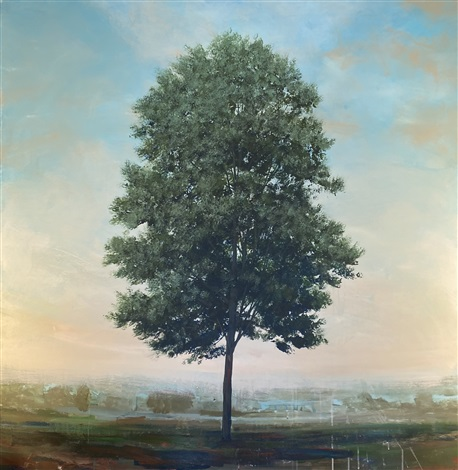
\includegraphics[width=8cm]{figures/peter-hoffer-spirit.jpg}
    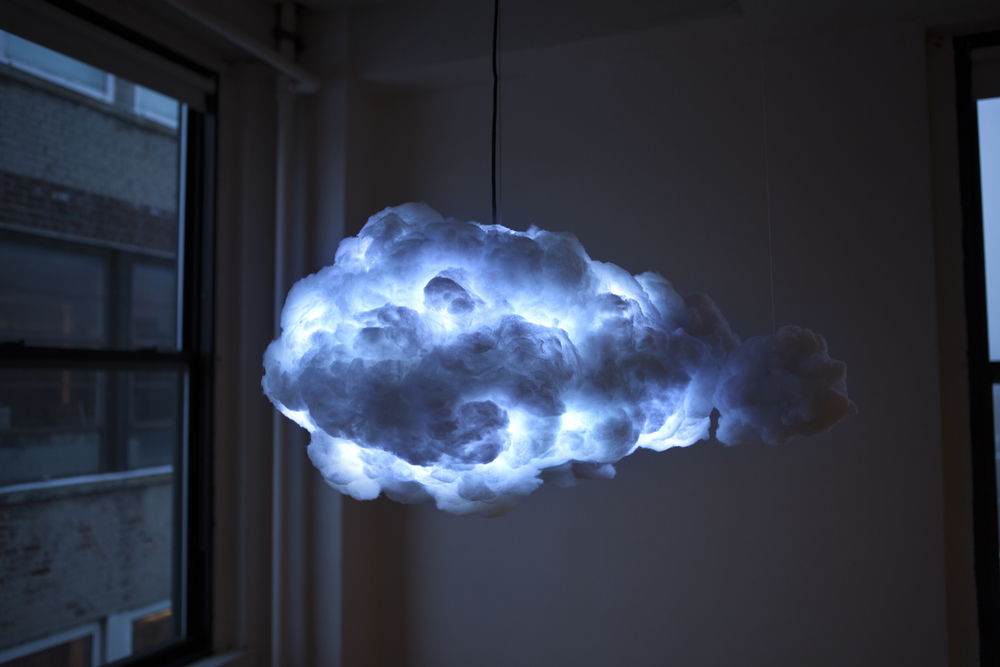
\includegraphics[width=8cm]{figures/cloud.jpg}
}
\caption{Left: \textit{Spirit}\cite{spirit} by Peter Hoffer, 2021; Right: \textit{The Cloud}\cite{thecloud} by Richard Clarkson.}
\end{figure}

\newpage{}

\section{Challenges}

From my early results in trying to implement the aforementioned paper, I have observed that generation of the initial octree is a slow process. I wish to extend the method to animated models rather than purely static meshes, so I will look at methods of quickly updating a preexisting octree to match transformed geometry.

I may also briefly explore the use of surface aligned volumetric textures as a potential alternative to the view aligned textures presented in the paper, as this would alleviate the need for an octree, and make animation much simpler. The parameterization of the surface would pose a challenge in this approach, as the noise function must then be mapped to the surface before it can be applied to a manifold.

Any algorithm which requires raytracing (as is the case with shadowing or emission) will also be greatly limited in performance by the number of samples of the noise functions which are required \cite{pavie:hal-02413269}, therefore another challenge will be to find ways to accelerate this process. One of the main benefits of using spot noise is how easily it can be controlled by artists, so rendering should at least be fast enough for immediate feedback to the artist if parameters are changed, even if real-time is not possible.

\section{Summary}

While I have given several possible directions for extending the work by Pavie et al. in this proposal, I expect that in the process of implementing the work further directions may present themselves. I believe that the technique of volumetric spot noise has much unexplored potential in achieving interesting textural effects.

\printbibliography

\end{document}
